\documentclass{article}
\usepackage[utf8]{inputenc}
\usepackage{amsmath}
\usepackage{amssymb}
\usepackage{amsfonts}
\usepackage{tikz}
\usepackage{pgfplots}
\pgfplotsset{compat=1.18}
\title{Euler's proof outline of the Basel problem}
\author{Dave Neary}
\date{April 2022}

\begin{document}

\maketitle

\section{Introduction}

The Basel problem was the name given to the question of whether there was a closed form for the convergent sum
\[ \sum_{n=1}^{\infty} \frac{1}{n^2} \]

It is named after the city of Basel, after the Bernoulli brothers Jacob and Johann, who were from there, and studied the problem at the 17th century, and also after Euler, who also lived in Basel, and who eventually came up with the surprising closed form:
\[ \sum_{n=1}^{\infty} \frac{1}{n^2}  = \frac{\pi^2}{6} \]

The following is a sketch outline of the derivation that Euler discovered, which relied on several assumptions which were not rigorously proven for another century.

\section{Convergence of $\sum \frac{1}{n^2}$}

There are a few ways to prove that $\sum \frac{1}{n^2}$ converges, we will use two methods, one
comparing the sum to a convergent telescoping series, and another relying on the integral test, which
we can use to establish bounds for the value of the final series sum.

First, by making the denominator smaller, we can make each term larger, and by adding this larger sum,
we can prove convergence. Note that, for $n>1$:
\[ \frac{1}{n^2} < \frac{1}{n(n-1)} = \frac{1}{n-1} - \frac{1}{n} \]
and therefore:

\begin{align*}
     \sum_{i=1}^{\infty} \frac{1}{n^2} &< 1 + \sum_{i=2}^{\infty} \frac{1}{n(n-1)} \\
     &= 1 + \sum_{i=2}^{\infty} \left(\frac{1}{n-1} - \frac{1}{n} \right) \\
     &= 2
\end{align*}

Similarly:
\[ \frac{1}{n^2} > \frac{1}{n(n+1)} = \frac{1}{n} - \frac{1}{n+1} \]

and summing over $n$ from 1 to $\infty$ gives a lower limit of 1 for the series. We thus have:
\[ 1 < \sum_{n=1}^{\infty} \frac{1}{n^2} < 2 \]

\section{Tightening the bounds using integration}

We can improve on these bounds using an integral method to estimate the "tail" of the series:
\[ \int_k^{\infty} \frac{dx}{x^2} < \sum_{n=k}^{\infty} \frac{1}{n^2} < \frac{1}{k^2} +  \int_k^{\infty} \frac{dx}{x^2} \]

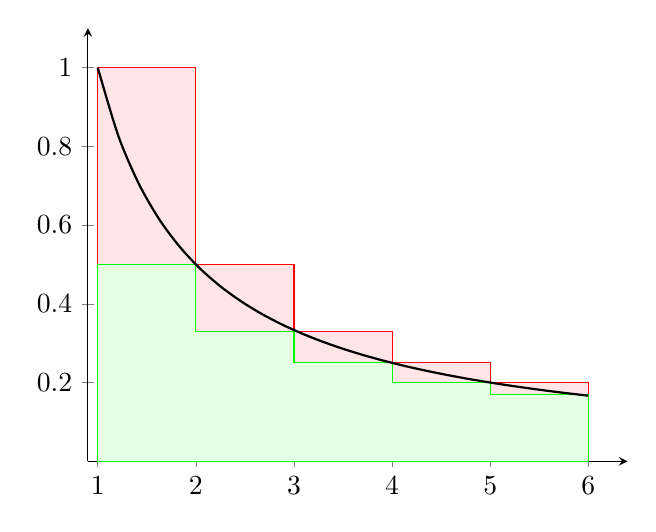
\begin{tikzpicture}
\begin{axis}[
    xtick={1,...,6},ytick={0.2,0.4,0.6,0.8,1.0},
    y=5cm, xmax=6.4,ymax=1.1,ymin=0,xmin=0.9,
    enlargelimits=true,
    axis lines=middle,
    clip=false
    ]
\addplot+[color=red,fill=red!10!white,const plot, mark=none]
    coordinates {(1,1) (2,0.5) (3,0.33) (4,0.25) (5,0.2) (6,0.17)}\closedcycle;
\addplot+[color=green,fill=green!10!white,const plot, mark=none]
    coordinates {(1,0.5) (2,0.33) (3,0.25) (4,0.2) (5,0.17) (6,0.14)}\closedcycle;
\addplot[smooth, thick,domain=1:6]{1/x};
\end{axis}
\end{tikzpicture}

As we can see above, the sum is equivalent to the left Riemann sum estimate for the integral of $f(x)$ (in the illustration, $f(x) = \frac{1}{x}$), while the sum except for the first term is the right Riemann sum. For $f(x)=\frac{1}{x^2}$, a monotonic decreasing function, the left Riemann sum is always bigger than the integral, and the right Riemann sum is smaller than the integral. Starting from $n=k$ gives the inequality above.

If we take out the first 4 terms of the series before we find the integral bounds, we get:
\begin{align*}
    \sum_{n=1}^{4} \frac{1}{n^2} + \int_5^{\infty} \frac{dx}{x^2} &&<&& \sum_{n=1}^{\infty} \frac{1}{n^2} &&<&& \sum_{n=1}^{5} \frac{1}{n^2} + \int_5^{\infty} \frac{dx}{x^2} \\
    \sum_{n=1}^{4} \frac{1}{n^2} + \left. \frac{-1}{x} \right|_{5}^{\infty} &&<&& \sum_{n=1}^{\infty} \frac{1}{n^2} &&<&& \sum_{n=1}^{5} \frac{1}{n^2} + \left. \frac{-1}{x} \right|_{5}^{\infty} \\
    \frac{205}{144} + \frac{1}{5} &&<&& \sum_{n=1}^{\infty} \frac{1}{n^2} &&<&& \frac{5269}{3600} + \frac{1}{5} \\
    1.6236 &&<&& \sum_{n=1}^{\infty} \frac{1}{n^2} &&<&& 1.6636 \\
\end{align*} 

However good we make these bounds, this does not get us any closer to a closed form for the sum. We will need to use another method.

\section{Euler's product form for $\sin(x)$}

The Fundamental Theorem of Algebra says that any polynomial of degree $n$ can be decomposed into $n$ linear factors, representing the (possibly complex) roots of the polynomial. That is:
\[ P(x) = a_0 + a_1x + \cdots + a_nx^n = a_n\prod_{i=1}^{n}(x-r_i) \]

Euler theorized that this theorem would extend to all functions, including those with infinite polynomial representations (incidentally, this would not be proven for another 100 years, but it is correct). Since $\sin(x)$ has roots at $x=n\pi, n \in \mathbb{Z}$, Euler wrote it as a product of those roots:
\begin{align*}
    \sin(x) &= A(\cdots)(x-2\pi)(x-\pi)(x)(x+\pi)(x+2\pi)(\cdots) \\
    &= Ax(x^2-\pi^2)(x^2-4\pi^2)(x^2-9\pi^2)(\cdots) \\
\end{align*}

To calculate the scaling factor $A$, Euler used the well known limit:
\[ \lim_{x\to 0} \frac{\sin(x)}{x} = 1 \]

\begin{align*}
    \frac{\sin(x)}{x} &= A(x^2-\pi^2)(x^2-4\pi^2)(x^2-9\pi^2)(\cdots) \\
    \lim_{x\to 0} \frac{\sin(x)}{x} &= A(-\pi^2)(-4\pi^2)(-9\pi^2)(\cdots) \\
    &= 1 \\
    A &= \frac{1}{(-\pi^2)(-4\pi^2)(-9\pi^2)(\cdots)}
\end{align*}

Substituting this into the expression for $\sin(x)$ we get:

\begin{align*}
     \sin(x) &= \frac{x(x^2-\pi^2)(x^2-4\pi^2)(x^2-9\pi^2)(\cdots)}{(-\pi^2)(-4\pi^2)(-9\pi^2)(\cdots)} \\
     &= x \left(\frac{x^2-\pi^2}{-\pi^2}\right)\left(\frac{x^2-4\pi^2}{-4\pi^2}\right)\left(\frac{x^2-9\pi^2}{-9\pi^2}\right) \left(\cdots\right)\\
     &= x\left(1-\frac{x^2}{\pi^2}\right)\left(1-\frac{x^2}{4\pi^2}\right)\left(1-\frac{x^2}{9\pi^2}\right)\left(\cdots\right) \\
     &= x\prod_{n=1}^{\infty} \left(1-\frac{x^2}{n^2\pi^2}\right)
\end{align*}

Euler's second insight was that if two polynomial forms of $\sin(x)$ were equivalent, that the coefficients of each term in the polynomial would also be equal. He then took the Taylor's series for $\sin(x)$:
\[ \sin(x) = \frac{x}{1!} - \frac{x^3}{3!} + \frac{x^5}{5!} - \frac{x^7}{7!} + \cdots \]

and he equated the coefficients for the $x^3$ term. When multiplied out, the product form gives:
\[ \sin(x) = x - \left(\sum_{n=1}^{\infty} \frac{1}{n^2\pi^2}\right) x^3 + O(x^5) \]

where $O(x^5)$ is a polynomial with $x^5$ as the lowest order term.

This is because the only way to get an $x^3$ term is to multiply the leading $x$ by exactly one of the $x^2$ terms in the product, and multiplying by $1$ for every other term in the product. By equating the coefficients of $x^3$ in both representations of $\sin(x)$, we get the result:

\begin{align*}
    -\frac{1}{6} &= -\sum_{n=1}^{\infty} \frac{1}{n^2 \pi^2}\\
    \frac{\pi^2}{6} &= \sum_{n=1}^{\infty} \frac{1}{n^2} \\
\end{align*}

\end{document}

